\documentclass[10pt,letterpaper]{article}
\usepackage[margin=0.75in,columnsep=0.28in]{geometry}
\usepackage[T1]{fontenc}
\usepackage{newtxtext,newtxmath}
\usepackage{graphicx,booktabs,multirow,xcolor,amsmath,microtype,tikz,enumitem,caption}
\usepackage[hidelinks]{hyperref}
\usetikzlibrary{positioning,fit,arrows.meta,calc}
\captionsetup{font=small,labelfont=bf}
\setlist{nosep,leftmargin=1.2em}
\definecolor{cblue}{HTML}{2a78d6}
\definecolor{corange}{HTML}{eb6834}
\definecolor{caqua}{HTML}{1baf7a}
\definecolor{cgray}{HTML}{8a8984}
\newcommand{\pct}[1]{#1\%}

\title{\Large\bfseries PickNet: One Transformer for Human Draft Picks\\in \emph{Magic: The Gathering}, Trained on 17 Sets}
\author{Zane Blanton\\[2pt]\small\texttt{zeblanton@gmail.com}\quad\small\url{https://github.com/zscore/mtg-open-lane}}
\date{\small October 2026}

\begin{document}
\twocolumn[
\begin{@twocolumnfalse}
\maketitle
\vspace{-1em}
\begin{abstract}\small
\noindent
We train PickNet, an 8.4M-parameter transformer that predicts which card a human drafter takes from a
\emph{Magic: The Gathering} booster pack. It is trained on 1.72M Premier and Traditional drafts from 17 sets of
17Lands data. The model reads the whole draft so far: every pack shown, every pick made, and the cards the
other seven drafters took from each pack that came back around the table. Candidate cards attend to each other
and to that history. One model covers every set. Cards are shared by name across sets, and a set embedding,
the drafter's rank and skill, and calendar time are added to every input token. On a chronological split, where
we test on the last 15\% of each format's drafts, PickNet agrees with the human pick on
\textbf{\pct{70.8}} of 13.8M test picks (\pct{68.5} excluding forced last picks). That is 1.3 points above our
best single-set model on the development set and 4--6 points above single-set baselines elsewhere. On the 8
sets it shares with puder, the strongest public model, PickNet scores \pct{70.8} against puder's
\pct{69.9} (log loss 0.749 against 0.778 nats), even though puder is scored on an easier random split. To get the \pct{69.9}, we re-scored puder's released model: its
reported \pct{71} counts padding slots as correct picks. Ablations show where the accuracy comes from. The
drafter's pool is worth about 15 points over a pick-order bot, the other cards in the pack about 3, and the
history of what was passed about 1. Strong drafters are easier to predict, by about 4 points.
The whole model trains in 14 hours on a 16\,GB laptop.
\end{abstract}
\vspace{1.5em}
\end{@twocolumnfalse}
]

% =====================================================================
\section{Introduction}

In a \emph{Magic: The Gathering} booster draft, eight players each open a pack of 13--15 cards, take one,
and pass the rest to the next player. This repeats until the packs are empty, three times with the passing
direction alternating, and each player then builds a 40-card deck from the 39--45 cards they took. Every pick
balances a card's raw strength against the colours and archetype the drafter is already in, and against what
the passed packs suggest the neighbours are taking.

Predicting the pick a human makes is the standard benchmark for draft AI~\cite{ward2021,bertram2021,draftfm}.
It is not the same as drafting \emph{well}, but a model that imitates strong humans is a usable drafting
assistant, a realistic opponent for simulating tables, and a source of the card ``affinities'' humans act on.
17Lands~\cite{17lands} publishes every pick of every draft its users record, with the pack contents, so the
problem now has millions of labelled examples per set.

Accuracy in this literature has settled around 66--71\% top-1. A pick-order bot (one rating per card) gets
about 50\%. Siamese and contrastive models get 67--69\% on a single set~\cite{bertram2024infonce},
an LLM fine-tuned with LoRA gets 66\%~\cite{urzagpt}, statistical-drafting gets about 70\% on top
players~\cite{statdraft}, and puder~\cite{puder}, a 7M-parameter transformer trained on about 2M drafts, reports 71\%.
Results are hard to compare: papers use different sets, random or chronological splits, all drafters or only
strong ones, and differently defined accuracy.

This report makes four contributions:
\begin{enumerate}
\item \textbf{A pick model that reads the table.} PickNet's history tokens include, for each pack that
returns, the cards the other seven drafters took from it. Candidates attend to each other, so the model can
learn which cards compete within a pack (\S\ref{sec:model}).
\item \textbf{One model for 17 sets, trained on a laptop.} Shared name ids, card features, a set embedding and
calendar time let a single 8.4M-parameter model train on 1.72M drafts. It reaches \pct{70.8} top-1
on 13.8M chronologically held-out picks (\S\ref{sec:results}).
\item \textbf{A like-for-like comparison with puder.} We re-score puder's released model and find
a scoring artefact worth 1.8 points. On the 8 sets both models cover, PickNet leads by 0.9 points on a
harder split (\S\ref{sec:puder}).
\item \textbf{Where the accuracy comes from.} Pool, pack and history ablations; accuracy by pick position and
drafter skill; and eight-bot table simulations (\S\ref{sec:analysis}).
\end{enumerate}

% =====================================================================
\section{Related work}

\textbf{Pick prediction.} Ward et al.~\cite{ward2021} introduced the benchmark on Draftsim M19 bot drafts:
an MLP over pool counts reached 48.7\% top-1. Bertram et al.\ framed picking as contextual preference
ranking with Siamese networks~\cite{bertram2021}, then moved to 17Lands data with general card
representations~\cite{bertram2024general}, a contextual InfoNCE loss (68.8\% on NEO)~\cite{bertram2024infonce}
and, at scale, 125M picks across every set to MH3~\cite{bertram2026}. UrzaGPT~\cite{urzagpt} fine-tunes a 7--8B LLM
(66.2\%). DraftFM~\cite{draftfm} trains a 1.6M-parameter discrete-choice model on 149M picks from 29 sets
using only card text and features, which lets it draft sets it has never seen (51--60\% top-1 on day zero).
PickNet's output layer is the same conditional logit~\cite{mcfadden}: a softmax over exactly the cards in the
pack.

\textbf{puder.} The closest model to ours is puder~\cite{puder}, a causal transformer over card-id tokens with
skill and date metadata, a deck-inclusion auxiliary head, and pack dropout. It is trained on about 2M drafts
from 19 sets on a random split and reports about 71\% top-1. Its author found that hiding pack contents cost
only 0.57\%. We adopt its deck head, its pooling of Premier and Traditional drafts, and its name-shared card
ids.

\textbf{Deck strength and tables.} DraftEncoder~\cite{draftencoder} predicts a drafted deck's win rate.
DraftRec~\cite{draftrec} trains one model on both picks and match outcomes in MOBA drafts. Neither models
what the other drafters at the table take. puder's history could in principle infer it from the packs
shown, but as far as we know PickNet is the first pick model given the cards the other seven drafters took as
an explicit input.

% =====================================================================
\section{Data}\label{sec:data}

\textbf{Source.} 17Lands public draft files~\cite{17lands} for 17 sets released between April 2023 and
2026: MOM, WOE, LCI, MKM, OTJ, BLB, DSK, FDN, DFT, TDM, FIN, EOE, TLA, SOS, ECL, MSH and TMT. We use Premier Draft
(against humans, best-of-one) and Traditional Draft (best-of-three) for every set that has it, and skip
Quick Draft, whose other seats are bots. That is 2.46M drafts and 32 (set, event) files. Packs hold
13, 14 or 15 picks depending on the set. Each row of the source data gives the cards in the pack, the
card taken, the drafter's rank, their 17Lands win-rate and games-played buckets, the draft time, and each
card's final main-deck rate for that drafter.

\textbf{What the others took.} A pack seen at pick $p$ returns 8 picks later, after the other seven
drafters have each taken one card. The difference between the two observations, minus the drafter's own
pick, is exactly the multiset of cards the table took. The data never names the other seven drafters, but this
difference shows what they took, and it is the raw material of ``reading signals''.

\textbf{Split.} Within each set and event, drafts are ordered by time: the first 70\% train, the next 15\%
validate, and the last 15\% test. Test drafts therefore come from the end of each format, when the
metagame has shifted from what the model trained on. This is harder than a random split (\S\ref{sec:puder}). We
report results on the Premier Draft test drafts of every set: 331k drafts and 13.8M picks. Validation for early
stopping uses 4,000 Premier drafts sampled across sets.

\textbf{Layout.} Every draft is stored in one fixed layout: 3 packs $\times$ 15 pick slots, up to 15 distinct
cards per pack token, with card ids global across sets. Sets with 13- or 14-card packs leave the trailing
slots empty and masked out of the loss and every metric. The 1.72M training drafts stream from 7.8\,GB of
memory-mapped arrays.

% =====================================================================
\section{Model}\label{sec:model}

\begin{figure}[t]
\centering
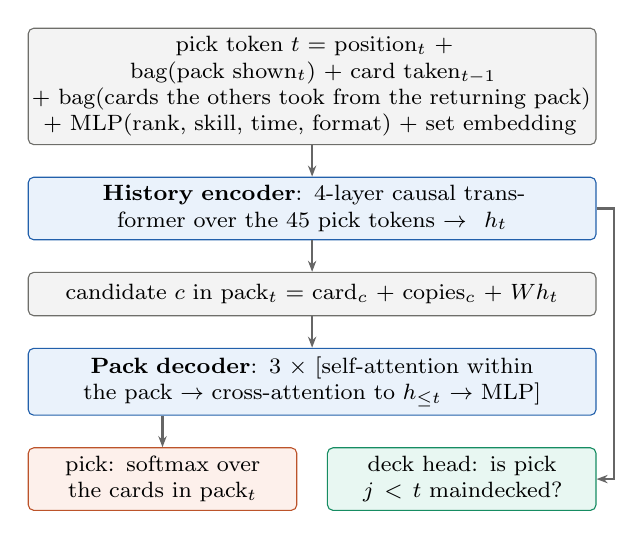
\begin{tikzpicture}[
  font=\footnotesize,
  box/.style={draw=#1!80!black,fill=#1!10,rounded corners=2pt,minimum height=0.55cm,inner sep=3pt,align=center,text width=7.0cm},
  box/.default=cgray,
  sm/.style={draw=#1!80!black,fill=#1!10,rounded corners=2pt,minimum height=0.55cm,inner sep=3pt,align=center,text width=3.2cm},
  arr/.style={-{Stealth[length=4pt]},draw=black!60,thick},
  node distance=0.4cm]
\node[box] (tok) {pick token $t$ = position$_t$ + bag(pack shown$_t$) + card taken$_{t-1}$\\
  + bag(cards the others took from the returning pack)\\ + MLP(rank, skill, time, format) + set embedding};
\node[box=cblue,below=of tok] (hist) {\textbf{History encoder}: 4-layer causal transformer over the 45 pick tokens $\to h_t$};
\node[box,below=of hist] (ctok) {candidate $c$ in pack$_t$ = card$_c$ + copies$_c$ + $W h_t$};
\node[box=cblue,below=of ctok] (cand) {\textbf{Pack decoder}: 3 $\times$ [self-attention within the pack $\to$ cross-attention to $h_{\le t}$ $\to$ MLP]};
\node[sm=corange,below=of cand.south west,anchor=north west] (pick) {pick: softmax over the cards in pack$_t$};
\node[sm=caqua,below=of cand.south east,anchor=north east] (deck) {deck head: is pick $j<t$ maindecked?};
\draw[arr] (tok) -- (hist);
\draw[arr] (hist) -- (ctok);
\draw[arr] (ctok) -- (cand);
\draw[arr] (cand.south -| pick.north) -- (pick.north);
\draw[arr] (hist.east) -- ++(0.22,0) |- (deck.east);
\end{tikzpicture}
\caption{PickNet. The history encoder summarises everything the drafter knew before pick $t$. Candidate
tokens for the cards in pack $t$ attend to each other (which cards compete) and to the history, and each
gets one logit. Card vectors are a learned per-name embedding plus a projection of fixed card features.}
\label{fig:arch}
\end{figure}

\textbf{Cards.} A card's vector is a learned embedding of its \emph{name}, plus a linear projection of a fixed
465-dimensional feature vector: colours, rarity, mana value, card types, Scryfall-derived pips, mana production,
power/toughness, keywords and rules-text roles, and a 384-dimensional \texttt{bge-small-en-v1.5}~\cite{bge}
embedding of the rules text with the card's own name masked. A reprint or basic land shares one learned vector
across sets while keeping set-specific features. Only about 220 of the 5,317 printings are shared across sets,
so most of what pooling buys is data, not shared cards.

\textbf{History encoder.} Pick $t$ gets one token (Fig.~\ref{fig:arch}): a position embedding; a projected,
count-weighted mean of the card vectors in the pack shown at $t$; the card taken at $t-1$; a projected
bag of the cards the other seven took from the pack that has just returned (zero for the first 8 picks of
each pack); an MLP of per-draft context; and a learned set embedding. Context is the drafter's rank
(one-hot), the 17Lands win-rate and games-played buckets, days since the format opened, calendar years since 2023,
a Traditional flag and the pack size. Time is continuous rather than a learned month token, because
chronological test drafts fall in months that no training draft covers. Causal self-attention over these 45 tokens
gives a state $h_t$ that has seen packs $\le t$ and picks $< t$: exactly what the drafter knew.

\textbf{Pack decoder.} Each card $c$ in pack $t$ becomes a candidate token: its card vector, an embedding of
how many copies are in the pack, and $W h_t$. Three pre-norm blocks alternate self-attention among the
candidates of the same pack, cross-attention to history states $\le t$, and an MLP. A small head gives one
logit per candidate, and the pick probability is a softmax over the cards actually in the pack.

\textbf{Deck head.} Following puder, a bilinear head scores, from each state $h_t$, whether each earlier
pick $j<t$ ends up in the final main deck. Its target is the 17Lands main-deck rate, with binary cross-entropy weighted by $(t+1)/T$,
and its loss weight is 0.3 relative to the pick NLL. We did not ablate it.

\textbf{Training.} $d=256$, 8 heads, 4 history layers, 3 pack blocks, dropout 0.05, 8.36M parameters.
AdamW (weight decay 0.01), batch 32 drafts, gradient clipping at 1, a one-cycle schedule of 53,791 steps
(one pass over the training drafts). Epoch 1 peaks at learning rate $5\!\times\!10^{-4}$. Epoch 2 starts from epoch 1's
best weights with a fresh cycle peaking at $2\!\times\!10^{-4}$ and a new shuffle. We keep the weights with the best
validation NLL. Training runs on an Apple-silicon laptop (16\,GB, PyTorch MPS) at 73 drafts/s, taking 7.6\,h and
6.8\,h for the two epochs. Two 25-minute pilots with and without puder's pack dropout (hiding the
shown pack and the others' picks from the history for 50\% of drafts) differed by 0.0002 top-1, so we turned
it off.

% =====================================================================
\section{Results}\label{sec:results}

\begin{table*}[t]
\centering\small
\caption{Test results by set, the same three metrics for every model. \emph{Top-1}: share of real picks where
the model's first choice is the human's pick. \emph{Non-forced}: the same, excluding picks with only one card
left. \emph{NLL}: mean negative log-likelihood of the human's pick (nats; lower is better). \emph{Rating} and
\emph{pool} are trained on that set alone, on the same chronological split as PickNet. puder is the released v1
model, re-scored on real picks of its own random-split Premier test drafts (\S\ref{sec:puder}), so its column
is not scored on the same drafts as the others. Bold: best in each row and metric.
$^a$The 8 sets puder covers, weighted by puder's test drafts per set (478 in total).
$^b$Weighted by test picks; the 14 sets that have single-set baselines, and all 17.}
\label{tab:sets}
\setlength{\tabcolsep}{4.2pt}
\begin{tabular}{lr cccc cccc cccc}
\toprule
 & test picks & \multicolumn{4}{c}{top-1 $\uparrow$} & \multicolumn{4}{c}{non-forced top-1 $\uparrow$} & \multicolumn{4}{c}{NLL $\downarrow$} \\
\cmidrule(lr){3-6}\cmidrule(lr){7-10}\cmidrule(lr){11-14}
set & (k) & rating & pool & puder & PickNet & rating & pool & puder & PickNet & rating & pool & puder & PickNet \\
\midrule
BLB & 904 & .452 & .659 & \textbf{.725} & .714 & .406 & .630 & \textbf{.702} & .690 & 1.425 & .915 & .736 & \textbf{.731} \\
DFT & 889 & .473 & .650 & -- & \textbf{.711} & .433 & .623 & -- & \textbf{.689} & 1.370 & .945 & -- & \textbf{.741} \\
DSK & 1056 & .475 & .665 & .711 & \textbf{.722} & .435 & .639 & .689 & \textbf{.700} & 1.358 & .901 & .737 & \textbf{.711} \\
ECL & 566 & .450 & .669 & -- & \textbf{.717} & .403 & .640 & -- & \textbf{.692} & 1.413 & .881 & -- & \textbf{.723} \\
EOE & 611 & .477 & .651 & -- & \textbf{.711} & .433 & .621 & -- & \textbf{.687} & 1.350 & .938 & -- & \textbf{.738} \\
FDN & 825 & .483 & .666 & .716 & \textbf{.724} & .443 & .640 & .695 & \textbf{.702} & 1.355 & .905 & .753 & \textbf{.708} \\
FIN & 884 & .466 & .651 & -- & \textbf{.709} & .425 & .624 & -- & \textbf{.687} & 1.391 & .942 & -- & \textbf{.745} \\
LCI & 911 & .468 & .643 & .679 & \textbf{.701} & .430 & .618 & .657 & \textbf{.679} & 1.412 & .969 & .810 & \textbf{.774} \\
MKM & 922 & .474 & .644 & .692 & \textbf{.706} & .430 & .614 & .666 & \textbf{.681} & 1.363 & .948 & .803 & \textbf{.751} \\
MOM & 1387 & -- & -- & .689 & \textbf{.701} & -- & -- & .666 & \textbf{.680} & -- & -- & .805 & \textbf{.769} \\
MSH & 432 & .497 & .644 & -- & \textbf{.699} & .459 & .617 & -- & \textbf{.676} & 1.324 & .954 & -- & \textbf{.775} \\
OTJ & 1230 & .497 & .652 & .697 & \textbf{.707} & .458 & .625 & .674 & \textbf{.684} & 1.317 & .934 & .788 & \textbf{.751} \\
SOS & 677 & .467 & .671 & -- & \textbf{.715} & .426 & .645 & -- & \textbf{.693} & 1.393 & .872 & -- & \textbf{.731} \\
TDM & 638 & .477 & .643 & -- & \textbf{.689} & .436 & .615 & -- & \textbf{.665} & 1.368 & .942 & -- & \textbf{.796} \\
TLA & 632 & .477 & .649 & -- & \textbf{.704} & .436 & .621 & -- & \textbf{.680} & 1.358 & .943 & -- & \textbf{.759} \\
TMT & 198 & -- & -- & -- & \textbf{.721} & -- & -- & -- & \textbf{.698} & -- & -- & -- & \textbf{.716} \\
WOE & 1044 & -- & -- & .684 & \textbf{.694} & -- & -- & .660 & \textbf{.670} & -- & -- & .790 & \textbf{.785} \\
\midrule
8 shared$^a$ &  & -- & -- & .699 & \textbf{.708} & -- & -- & .676 & \textbf{.686} & -- & -- & .778 & \textbf{.749} \\
14 sets$^b$ &  & .474 & .654 & -- & \textbf{.710} & .433 & .627 & -- & \textbf{.687} & 1.371 & .928 & -- & \textbf{.744} \\
all 17$^b$ & 13807 & -- & -- & -- & \textbf{.708} & -- & -- & -- & \textbf{.685} & -- & -- & -- & \textbf{.749} \\
\bottomrule
\end{tabular}

\end{table*}

\begin{figure}[t]
\centering
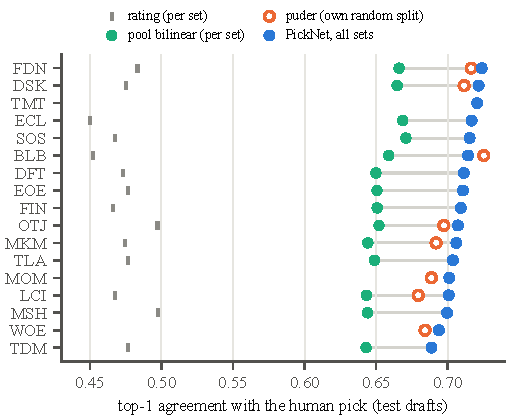
\includegraphics[width=\columnwidth]{figs/per_set.pdf}
\caption{Test top-1 by set, sorted by PickNet's score. Grey lines join each set's single-set pool model to
the all-sets PickNet. Rating bots sit near 0.47 on every set.}
\label{fig:sets}
\end{figure}

Table~\ref{tab:sets} reports top-1, non-forced top-1 and NLL for every model on every set, and
Fig.~\ref{fig:sets} plots the top-1 column. Weighted by picks, PickNet agrees with the human on \textbf{70.8\%} of
13.8M test picks. Excluding forced picks it agrees on 68.5\%, and its NLL is 0.749 nats per pick. Per set, top-1
ranges from 68.9\% (TDM) to 72.4\% (FDN). On the 14 sets with single-set baselines, PickNet beats the bilinear pool
model on every set and every metric: 71.0\% against 65.4\% top-1, 68.7\% against 62.7\% non-forced, and 0.744
against 0.928 nats. The rating bot scores 47.4\%, 43.3\% and 1.371. On MSH, our development set, it gains 1.3 points (68.6\% $\to$ 69.9\%) over the best
single-set PickNet, a 3.9M-parameter model with the same architecture minus set pooling. On FDN, the other set
with a single-set PickNet, it gains 1.2 points (71.2\% $\to$ 72.4\%). Epoch 2 improved every set by 0.2--0.4 points over
epoch 1 (70.5\% overall). Validation accuracy was still rising slowly at the end of epoch 2 (Fig.~\ref{fig:curve}).

\begin{figure}[t]
\centering
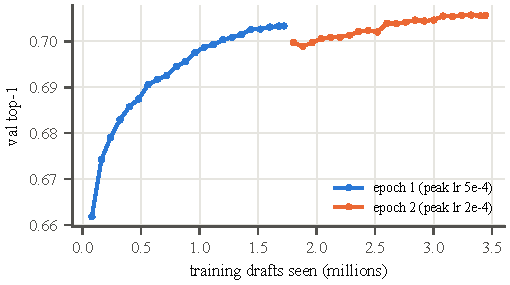
\includegraphics[width=\columnwidth]{figs/train_curve.pdf}
\caption{Validation top-1 (4,000 Premier drafts across all sets) over two passes of the 1.72M training drafts.}
\label{fig:curve}
\end{figure}

\subsection{Comparison with puder}\label{sec:puder}

puder's released model ships with its 1,024 test drafts. Re-scoring it on them, we reproduce its reported
accuracy formula (71.3\%) but find that the formula counts padding as correct. Every draft is 45 slots long,
so sets with 13- or 14-card packs leave 3 or 6 empty slots. On those slots every logit is $-\infty$, the
argmax returns index 0, and index 0 is the padding token, so each empty slot scores as a correct pick. 756
of the 1,024 test drafts have padding. Counting real picks only, puder scores \textbf{69.5\%} (69.2\% on its
Premier drafts). puder's input also includes the draft's final win--loss record, which isn't known at pick
time, but shuffling it across drafts moves accuracy by only $-$0.03 points.

Eight of puder's sets are in our data. Table~\ref{tab:sets} scores puder on its own Premier test drafts from
those sets with the same three metrics we use, weighting the 8-set average by its 478 test drafts. PickNet leads
on all three: \textbf{70.8\%} against \textbf{69.9\%} top-1, 68.6\% against 67.6\% non-forced, and 0.749 against 0.778
nats. It is ahead on 7 of the 8 sets by top-1 and by non-forced top-1, and on all 8 by NLL. The exception is BLB,
where puder has only 57 test drafts. The NLL gap (0.03 nats) is relatively larger than the top-1 gap: PickNet
puts more probability on the human's pick overall, not just more often ranks it first.
The comparison is not head to head:
\begin{itemize}
\item \textbf{Different test drafts.} puder's random split almost certainly trains on our test drafts, so it
can't be scored on them. Its per-set figures rest on 45--73 drafts each, so its 8-set average has a
standard error of about 0.4 points.
\item \textbf{Different splits.} puder's test drafts come from the same weeks as its training drafts. Ours come
from the end of each format, after the metagame has shifted. That handicaps PickNet, so a 0.9-point lead on
the harder test is, if anything, an underestimate.
\end{itemize}
The clean comparison would be to retrain puder's code on our split. A practical difference: puder's final
run took 51 GPU-hours on a desktop GPU, and PickNet's two epochs took 14 hours on a laptop.

% =====================================================================
\section{Analysis}\label{sec:analysis}

\begin{table}[t]
\centering\small
\caption{What context buys, MSH test (10,292 drafts, 432k picks). All rows except the last two are trained
on MSH alone (or, for multiset rows, 7 other sets $\pm$ MSH, 20k drafts each). NF: non-forced picks.}
\label{tab:ablate}
\setlength{\tabcolsep}{3.2pt}
\begin{tabular}{lrccc}
\toprule
model & params & NLL & top-1 & NF \\
\midrule
rating: one number per card & 340 & 1.324 & .497 & .459 \\
pool: + rank-32 card$\times$pool bilinear & 26k & .954 & .644 & .617 \\
+ candidates attend within the pack & 0.57M & .855 & .673 & .647 \\
+ causal history (PickNet) & 1.3M & .826 & .682 & .658 \\
PickNet, $d$=192 & 3.9M & .815 & .686 & .662 \\
\midrule
features only, 7 other sets (day zero) & 1.4M & 1.411 & .508 & .470 \\
features only, 7 other sets + MSH & 1.4M & .810 & .686 & .661 \\
\midrule
\textbf{PickNet, all 17 sets} & 8.4M & \textbf{.775} & \textbf{.699} & \textbf{.676} \\
\textit{DraftFM, MSH day zero~\cite{draftfm}} & 1.6M & 1.135 & .567 & .534 \\
\bottomrule
\end{tabular}
\end{table}

\textbf{Context is worth 18 points.} Table~\ref{tab:ablate} builds the model up on MSH. A pick-order
bot agrees with humans half the time. Conditioning on the pool (staying in your colours) adds 15 points.
Letting the candidates attend to each other, so the model knows which cards compete, adds 3. The causal history
of passed packs and returning picks adds 1 point (0.029 nats), most of it in pack 3 (66.3\% $\to$ 67.6\%), when
the drafter has seen the most of the table. Pooling all 17 sets adds 1.3 points on top of the largest
single-set model.

This also resolves puder's finding that pack contents barely matter. Hiding the shown pack from the
\emph{history} (puder's pack dropout) made no difference in our pilots either. The 3 points come from
candidate-to-candidate attention: the model compares the cards in front of the drafter, which is a
different use of the pack.

\textbf{Day zero is a different problem.} Without card ids, trained only on 7 other sets, the model scores
50.8\% on MSH, barely above a rating bot fitted on MSH itself. DraftFM, with 4$\times$ the sets and about 25$\times$ the
picks, reaches 56.7\%. The same features-only model trained with MSH's training drafts as well reaches 68.6\%,
matching the largest id-based single-set model. Card features generalise well once a set has data, but rules
text alone is a poor guide to card strength.

\begin{figure}[t]
\centering
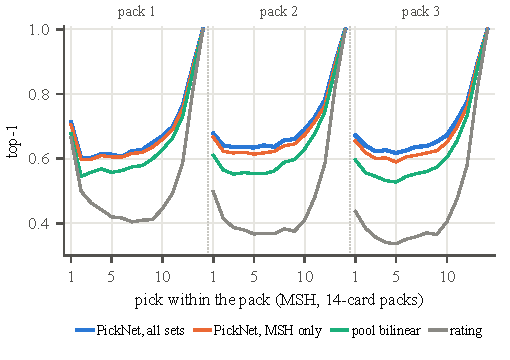
\includegraphics[width=\columnwidth]{figs/by_pick.pdf}
\caption{Test top-1 by pick position, MSH. Every model is near-perfect at the end of a pack, where few or
no choices remain. The gap to the rating bot is widest in mid-pack, where context matters most.}
\label{fig:bypick}
\end{figure}

\textbf{Where in the draft.} Fig.~\ref{fig:bypick} shows the familiar U shape~\cite{ward2021}. First picks
are relatively predictable (71\% for PickNet), since they depend only on card quality and the format's
consensus. The hardest picks are 2--8 of each pack, and that is where context models beat the rating bot by
the most: 24 points on picks 3--8. PickNet's advantage over the single-set model is largest in packs 2 and 3
(+1.5 and +1.9 points against +0.7 in pack 1), when there is a pool to condition on.

\begin{table}[t]
\centering\small
\caption{MSH test top-1 by drafter tier (17Lands win-rate and games-played buckets).}
\label{tab:tiers}
\setlength{\tabcolsep}{3.5pt}
\begin{tabular}{lrccc}
\toprule
tier & drafts & rating & MSH-only & all sets \\
\midrule
all drafters & 10,292 & .497 & .686 & \textbf{.699} \\
win rate $<$ 50\% & 2,638 & .485 & .671 & \textbf{.684} \\
Mythic rank & 1,636 & .504 & .701 & \textbf{.716} \\
win rate $\geq$ 60\% & 2,561 & .509 & .700 & \textbf{.712} \\
win rate $\geq$ 62\%, $\geq$100 games & 840 & .512 & .711 & \textbf{.722} \\
\bottomrule
\end{tabular}
\end{table}

\textbf{Strong drafters are more predictable} (Table~\ref{tab:tiers}). PickNet agrees with drafters
whose 17Lands win rate is at least 62\% over 100+ games on 72.2\% of picks, against 68.4\% for drafters below 50\%.
The rating bot barely moves across tiers (48.5\% $\to$ 51.2\%). Strong players agree with each other about
\emph{context} (what fits this pool, given this pack) more than about raw card quality. Pooling sets helps
every tier by a similar 1.1--1.5 points. One caveat: 17Lands computes the win-rate bucket over the
drafter's whole history on the set, including the test weeks, and PickNet takes it as an input. That slightly
flatters the tier slices, though not the overall numbers.

\begin{table}[t]
\centering\small
\caption{Eight copies of a model drafting real opened MSH packs (1,000 tables, sampling at temperature 1),
compared with real test drafts. These are single-set MSH models. ATA: average pick taken; on-colour:
pack-3 picks in the drafter's top two colours (humans: 0.815); TV: total-variation distance of colour-pair
shares from humans.}
\label{tab:sim}
\setlength{\tabcolsep}{3.2pt}
\begin{tabular}{lcccccc}
\toprule
bots & ATA $r$ & wheel $r$ & on-colour & pair TV & P1P1 $r$ \\
\midrule
rating & \textbf{.989} & .984 & .559 & .150 & .875 \\
pool & .987 & \textbf{.988} & .773 & .122 & .954 \\
PickNet & .979 & .954 & \textbf{.802} & \textbf{.066} & \textbf{.973} \\
\bottomrule
\end{tabular}
\end{table}

\textbf{Simulated tables.} We seat eight copies of a model at a table, give them a real test drafter's
opened packs, and let each sample its pick from the softmax (Table~\ref{tab:sim}). Rating bots match per-card
statistics best (average pick taken, how often a card wheels), because a per-card rating is fitted to exactly
those marginals. But they don't draft like people: only 56\% of their pack-3 picks are in their two main
colours, against 81.5\% for humans. PickNet bots commit like humans (80\%), choose first picks like humans
($r=0.97$) and land on human-like colour pairs (TV 0.066). Every bot under-drafts the format's most popular
pair, though: WU is 23\% of real MSH drafters, 17\% of PickNet bots and 11\% of rating bots. Humans converge
on the best archetype harder than a model that imitates one pick at a time. Sharpening the sampling to
temperature 0.7 doesn't fix this (WU 19\%), and it makes the bots over-commit (0.828 on-colour).

% =====================================================================
\section{Limitations}

\begin{itemize}
\item \textbf{Imitation, not optimisation.} PickNet predicts what 17Lands users take, and 17Lands users skew
above the Arena average. Agreeing with them is not the same as drafting well. Skill conditioning
(setting the context to a top-tier drafter at inference time) is the obvious lever, and we haven't evaluated it.
\item \textbf{Comparisons across papers are loose.} Sets, splits and accuracy definitions differ. The
puder comparison is the most careful one here, and it is still not on identical test drafts.
\item \textbf{Single runs.} We report one seed. With 13.8M test picks, sampling error is negligible
($\pm$0.03 points, 95\% interval, resampling drafts), but run-to-run variation from training is not measured. The deck head and the
calendar-time feature were not ablated individually.
\item \textbf{New sets.} The id-based model needs a set's own drafts. On day zero, the features-only model is the
fallback, and it is far weaker (\S\ref{sec:analysis}).
\end{itemize}

\section{Conclusion}

A single transformer that reads the whole draft (the drafter's packs, picks, and what the rest of the table
took), trained on every set at once, predicts human picks better than any model trained on one set, and better
than the strongest public model on the sets they share. The accuracy comes mostly from the pool, then from
comparing the cards in the pack, and only a little from reading the table. Pooling sets is worth about
another point over the best single-set model. The training runs on a laptop overnight. Code, results and the
per-set test predictions are available at \url{https://github.com/zscore/mtg-open-lane}.

\small
\begin{thebibliography}{99}\setlength{\itemsep}{1pt}
\bibitem{17lands} 17Lands. Public datasets. \url{https://www.17lands.com/public_datasets}.
\bibitem{ward2021} H.~N. Ward, B.~Mills, D.~J. Brooks, A.~S. Khakhalin, D.~Troha. AI solutions for drafting in
\emph{Magic: the Gathering}. \emph{IEEE Conference on Games}, 2021. arXiv:2009.00655.
\bibitem{bertram2021} T.~Bertram, J.~F\"urnkranz, M.~M\"uller. Predicting human card selection in
\emph{Magic: The Gathering} with contextual preference ranking. \emph{IEEE CoG}, 2021. arXiv:2105.11864.
\bibitem{bertram2024general} T.~Bertram, J.~F\"urnkranz, M.~M\"uller. Learning with generalised card
representations for \emph{Magic: The Gathering}. \emph{IEEE CoG}, 2024. arXiv:2407.05879.
\bibitem{bertram2024infonce} T.~Bertram, J.~F\"urnkranz, M.~M\"uller. Contrastive learning of preferences
with a contextual InfoNCE loss. arXiv:2407.05898, 2024.
\bibitem{bertram2026} T.~Bertram, J.~F\"urnkranz, M.~M\"uller. Drafting \emph{Magic: The Gathering} with
high-dimensional card embeddings. \emph{IEEE Transactions on Games} 18(3), 2026. doi:10.1109/TG.2025.3646029.
\bibitem{urzagpt} T.~Bertram. UrzaGPT: LoRA-tuned large language models for card selection in collectible card
games. arXiv:2508.08382, 2025.
\bibitem{draftfm} B.~Ward. DraftFM: a foundation model for day-zero drafting in \emph{Magic: The Gathering}.
arXiv:2608.19568, 2026.
\bibitem{puder} P.~Czerner. puder: an AI for MTG drafting. \url{https://nicze.de/philipp/articles/puder/}, 2025;
code at \url{https://github.com/suyjuris/puder}.
\bibitem{statdraft} D.~J. Brooks. Statistical Drafting. \url{https://statisticaldrafting.com}, 2024.
\bibitem{draftencoder} A.~Rigaux, H.~Kashima. Predicting drafted deck strength for \emph{Magic: The
Gathering}. \emph{IEEE CoG}, 2026. arXiv:2607.04782.
\bibitem{draftrec} H.~Lee, D.~Hwang, H.~Kim, B.~Lee, J.~Choo. DraftRec: personalized draft recommendation for
winning in multi-player online battle arena games. \emph{WWW}, 2022. arXiv:2204.12750.
\bibitem{mcfadden} D.~McFadden. Conditional logit analysis of qualitative choice behavior. In \emph{Frontiers
in Econometrics}, 1974.
\bibitem{bge} S.~Xiao, Z.~Liu, P.~Zhang, N.~Muennighoff. C-Pack: packaged resources to advance general Chinese
embedding. arXiv:2309.07597, 2023.
\end{thebibliography}

\end{document}
